% !TEX program = pdflatex
% ------------------------------------------------------------
% ITKA2004 Databases & Data Management
% Lecture: Section 6 (Warehousing + Distribution + Paradigms) (90 min)
% Theme: metropolis (TikZ/LaTeX-only figures)
% Michael Emmerich, Professor of Intelligent Computing, PS Fellow
% Faculty of Information Technology, University of Jyväskylä
% ------------------------------------------------------------
\documentclass[10pt,aspectratio=169]{beamer}

\usetheme[
  progressbar=frametitle,
  numbering=fraction
]{metropolis}

% --- Packages
\usepackage[T1]{fontenc}
\usepackage[utf8]{inputenc}
\usepackage{amsmath,amssymb}
\usepackage{booktabs}
\usepackage{xcolor}
\usepackage{tikz}
\usetikzlibrary{positioning,arrows.meta,shapes.geometric,calc,fit}
% stick students
\newcommand{\stick}[3]{% x,y,headsymbol
  \begin{scope}[shift={(#1,#2)}]
    \draw[line width=0.9pt] (0,0.25) circle (0.18);
    \node[font=\scriptsize] at (0,0.25) {#3};
    \draw[line width=0.9pt] (0,0.07) -- (0,-0.55);
    \draw[line width=0.9pt] (-0.32,-0.15) -- (0.32,-0.15);
    \draw[line width=0.9pt] (0,-0.55) -- (-0.28,-0.95);
    \draw[line width=0.9pt] (0,-0.55) -- (0.28,-0.95);
  \end{scope}
}
% --- JYU-ish colors (adjust if you have official codes)
\definecolor{JYUblue}{HTML}{003A70}
\definecolor{JYUorange}{HTML}{FF6A00}

% --- Metropolis palette / accents
\setbeamercolor{palette primary}{bg=JYUblue, fg=white}
\setbeamercolor{frametitle}{bg=JYUblue!6, fg=JYUblue}
\setbeamercolor{progress bar}{fg=JYUorange, bg=JYUblue!20}
\setbeamercolor{structure}{fg=JYUblue}
\setbeamercolor{alerted text}{fg=JYUorange}
\setbeamercolor{title}{fg=JYUblue}
\setbeamercolor{subtitle}{fg=JYUblue!85}

% --- Blocks: blue for theory, orange for examples
\setbeamercolor{block title}{bg=JYUblue, fg=white}
\setbeamercolor{block body}{bg=JYUblue!5, fg=black}
\setbeamercolor{block title example}{bg=JYUorange, fg=white}
\setbeamercolor{block body example}{bg=JYUorange!10, fg=black}
\newenvironment{examplebox}[1][Example]{\begin{exampleblock}{#1}}{\end{exampleblock}}

% ------------------------------------------------------------
% Footer (Metropolis)
% ------------------------------------------------------------
\setbeamertemplate{frame footer}{%
  \tiny Michael Emmerich (Professor of Intelligent Computing, PS Fellow)\hfill Databases Spring 2026\hfill Faculty of Information Technology, University of Jyväskylä%
}

% --- Metadata
\title{Databases and Data Management}
\subtitle{Section 6: Warehousing, Distribution, and Database Paradigms}
\author{Michael Emmerich (Professor of Intelligent Computing, PS Fellow)}
\institute{Faculty of Information Technology\\University of Jyväskylä}
\date{Spring 2026}

% --- Title graphic (TikZ)
\titlegraphic{%
  \begin{tikzpicture}[remember picture,overlay]
    \node[anchor=south east,opacity=0.10] at ([xshift=-2mm,yshift=2mm]current page.south east) {%
      \begin{tikzpicture}[scale=0.75]
        \draw[rounded corners=6pt,line width=2pt] (0,0) rectangle (5,3);
        \draw[line width=2pt] (0.6,2.4) -- (4.4,2.4);
        \node[text=JYUblue] at (2.5,1.55) {\Large DW};
        \node[text=JYUblue] at (2.5,0.95) {\large NoSQL};
      \end{tikzpicture}
    };
  \end{tikzpicture}%
}

% --- TikZ styles
\tikzset{
  box/.style={draw,rounded corners,align=center,inner sep=4pt},
  soft/.style={draw,rounded corners,fill=black!3,align=center,inner sep=4pt},
  big/.style={draw,rounded corners,fill=JYUblue!6,align=center,inner sep=6pt},
  arr/.style={-Latex,thick},
}

\begin{document}

\maketitle


\begin{frame}{Core abbreviations (used throughout)}
\small
\begin{tabular}{@{}p{2.2cm}p{11.8cm}@{}}
\toprule
\textbf{Abbrev.} & \textbf{Meaning} \\
\midrule
DBMS & Database Management System \\
DW & Data Warehouse \\
ETL & Extract--Transform--Load \\
OLTP & Online Transaction Processing (operational databases) \\
OLAP & Online Analytical Processing (analytics / reporting) \\
NoSQL & \textbf{Not only SQL} (non-relational paradigms and systems) \\
CAP & Consistency--Availability--Partition tolerance (distributed trade-off intuition) \\
BASE & Basically Available, Soft state, Eventually consistent \\
\bottomrule
\end{tabular}
\end{frame}
% ============================================================
\begin{frame}{Today (90 minutes)}
\begin{itemize}
  \item Data warehousing: purpose, ETL, staging area, data marts
  \item OLTP vs Data Warehouse (why schemas and workloads differ)
  \item Distribution: three-tier architecture and parallel hardware architectures
  \item Replication vs sharding (and common replication configurations)
  \item Database paradigms: object(-relational) and NoSQL families
  \item BASE/CAP intuition and polyglot persistence
\end{itemize}
\end{frame}

\begin{frame}{Learning goals}
After this lecture you can:
\begin{enumerate}
  \item explain what a data warehouse is and what ETL does
  \item sketch a typical DW architecture and identify staging area + marts
  \item compare OLTP and DW workloads and schema style
  \item explain three-tier architecture and why it replaced file-server style
  \item distinguish shared-disk vs shared-nothing vs shared-memory
  \item explain replication vs sharding and master-slave vs peer-to-peer
  \item name major database paradigms beyond relational and when to use them
\end{enumerate}
\end{frame}

\begin{frame}{Outline}
\tableofcontents
\end{frame}

% ============================================================
\section{Data Warehousing}

\begin{frame}{What is data warehousing?}
\begin{block}{Definition (practical)}
Data warehousing is the systematic and periodic copying, transforming,
and refining of data from multiple sources into an environment for analysis.
\end{block}
\begin{itemize}
  \item Operational DBs support daily business (Online Transaction Processing, OLTP).
  \item Other applications: Production management, Public health monitoring
  \item Managers/analysts need historical, integrated, cross-system views.
  \item A data warehouse enables reporting, OLAP analysis, and data mining.
\end{itemize}
\end{frame}

\begin{frame}{Data warehouse architecture (ETL + marts)}
\centering
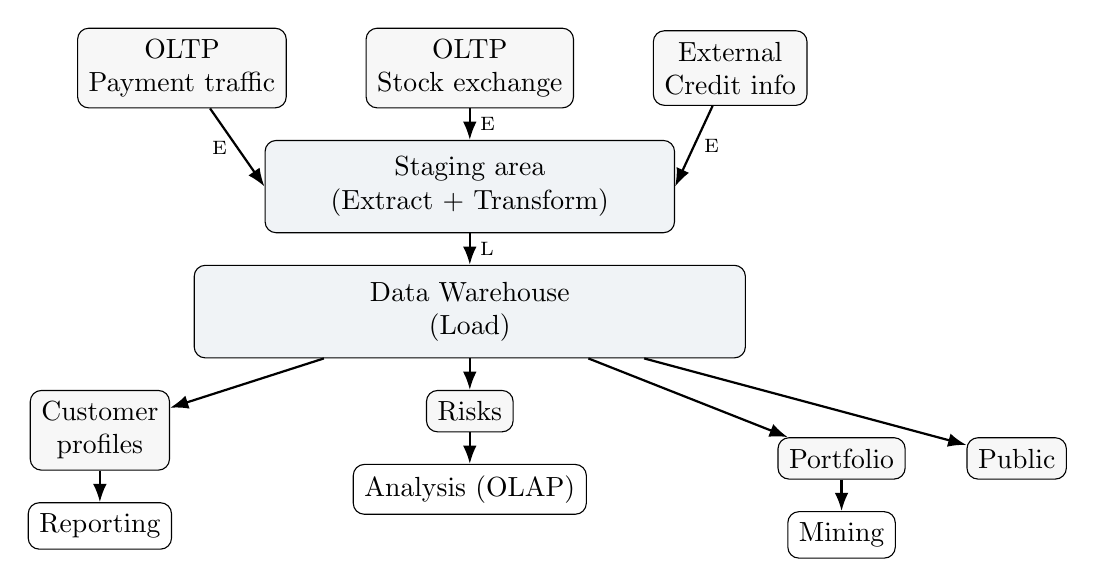
\begin{tikzpicture}[node distance=8mm]
% sources
\node[soft] (oltp1) {OLTP\\Payment traffic};
\node[soft, right=10mm of oltp1] (oltp2) {OLTP\\Stock exchange};
\node[soft, right=10mm of oltp2] (ext) {External\\Credit info};

% staging
\node[big, below=4mm of oltp2, minimum width=5.2cm] (staging) {Staging area\\(Extract + Transform)};
% arrows E,T
\draw[arr] (oltp1) -- node[left, font=\scriptsize]{E} (staging.west);
\draw[arr] (oltp2) -- node[right, font=\scriptsize]{E} (staging);
\draw[arr] (ext)   -- node[right, font=\scriptsize]{E} (staging.east);

% warehouse
\node[big, below=4mm of staging, minimum width=7.0cm, minimum height=8mm] (dw) {Data Warehouse\\(Load)};
\draw[arr] (staging) -- node[right, font=\scriptsize]{L} (dw);

% marts
\node[soft, below left=4mm and 3mm of dw] (m1) {Customer\\profiles};
\node[soft, below=4mm of dw] (m2) {Risks};
\node[soft, below right=10mm and 4mm of dw] (m3) {Portfolio};
\node[soft, below right=10mm and 28mm of dw] (m4) {Public};

\draw[arr] (dw) -- (m1);
\draw[arr] (dw) -- (m2);
\draw[arr] (dw) -- (m3);
\draw[arr] (dw) -- (m4);

% consumers
\node[box, below=4mm of m1] (rep) {Reporting};
\node[box, below=4mm of m2] (ana) {Analysis (OLAP)};
\node[box, below=4mm of m3] (min) {Mining};

\draw[arr] (m1) -- (rep);
\draw[arr] (m2) -- (ana);
\draw[arr] (m3) -- (min);

\end{tikzpicture}
\end{frame}

\begin{frame}{Staging area: why it exists}
\begin{itemize}
  \item Data is extracted from heterogeneous sources.
  \item Transformations in staging:
  \begin{itemize}
    \item unify formats and codes
    \item filter erroneous/poor-quality data
    \item derive new attributes (business logic)
  \end{itemize}
  \item Data is loaded periodically (batch): weekly, quarterly, etc.
  \item Sometimes corrected data is fed back into source systems.
\end{itemize}
\end{frame}

\begin{frame}{Data marts}
\begin{block}{Idea}
A data mart is a slice of the warehouse built for specific information needs
(department, geography, sensitivity, aggregation level, etc.).
\end{block}
\begin{itemize}
  \item Physical DB or logical (views).
  \item Helps access control and comprehension.
  \item Two common schools:
  \begin{itemize}
    \item marts built from warehouse (Inmon style)
    \item marts may combine warehouse + other data (Kimball style)
  \end{itemize}
\end{itemize}
\end{frame}

\begin{frame}{Star vs snowflake vs starflake (schema intuition)}
\small
\begin{columns}[T,onlytextwidth]
\column{0.47\textwidth}
\begin{block}{Fact + dimensions}
\begin{itemize}
  \item Fact table: events + measures (e.g., orders, transfers, includes keys of dimension tables and supports aggregation queries, e.g. sales total sales for customer and time period)
  \item Dimension tables: descriptive entities (product, customer, time)
\end{itemize}
\end{block}
\begin{examplebox}[Models]
\begin{itemize}
  \item \textbf{Star}: dimensions less normalized
  \item \textbf{Snowflake}: dimension tables normalized (e.g., BCNF)
\end{itemize}
\end{examplebox}

\column{0.50\textwidth}
\centering
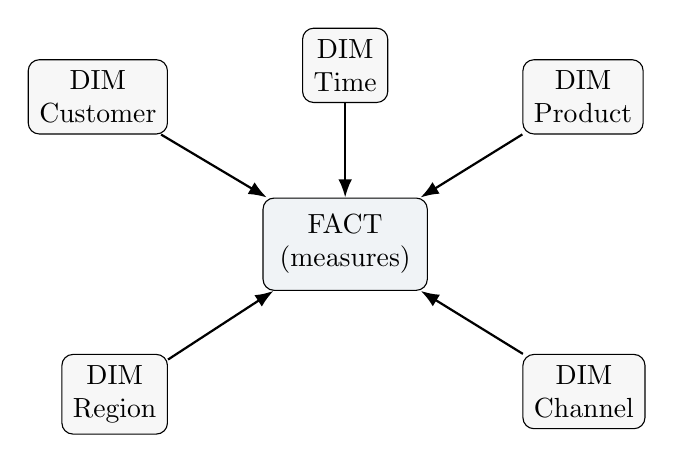
\begin{tikzpicture}[node distance=6mm]
\node[big] (fact) {FACT\\(measures)};
\node[soft, above left=8mm and 12mm of fact] (d1) {DIM\\Customer};
\node[soft, above=12mm of fact] (d2) {DIM\\Time};
\node[soft, above right=8mm and 12mm of fact] (d3) {DIM\\Product};
\node[soft, below left=8mm and 12mm of fact] (d4) {DIM\\Region};
\node[soft, below right=8mm and 12mm of fact] (d5) {DIM\\Channel};
\draw[arr] (d1) -- (fact);
\draw[arr] (d2) -- (fact);
\draw[arr] (d3) -- (fact);
\draw[arr] (d4) -- (fact);
\draw[arr] (d5) -- (fact);
\end{tikzpicture}
\end{columns}
\end{frame}

\begin{frame}{OLTP vs Data Warehouse (summary table)}
\scriptsize
\begin{tabular}{@{}p{3.2cm}p{5.4cm}p{5.2cm}@{}}
\toprule
 & \textbf{Operational DB (OLTP)} & \textbf{Data Warehouse} \\
\midrule
Purpose & Daily business & Analysis, planning, problem solving \\
Data source & Applications, users & Multiple source databases \\
Granularity & Precise & Aggregated + precise history \\
Nature & Dynamic snapshot & Static history, aggregation \\
Queries & Simple, few rows & Complex, aggregating \\
Writes & Small, frequent & Batch runs (large, periodic) \\
Indexes & Few & Many \\
Normal form & Highly normalized & Often denormalized \\
Users & Most Users & Subset (analysts, managers) \\
\bottomrule
\end{tabular}
\end{frame}

\begin{frame}{Master data (SOE vs SOR)}
\begin{block}{Master data}
Central information gathered in one place to ensure correctness and sharing.
\end{block}
\begin{itemize}
  \item \textbf{SOE (system of entry)}: accepted source(s) of data
  \item \textbf{SOR (system of record)}: the one correct version
\end{itemize}

\begin{examplebox}[Three implementation styles (sketch)]
\begin{itemize}
  \item Downstream: integrate from SOEs \(\rightarrow\) master DB as SOR
  \item Hub: one system is the SOE+SOR, feed others
  \item Enterprise: master DB is both SOE+SOR, source updates must pass integration
\end{itemize}
\end{examplebox}
\end{frame}
\begin{frame}{Master data example: one customer, many systems}
\small
\begin{columns}[T,onlytextwidth]
\column{0.53\textwidth}
\begin{examplebox}[Scenario]
A customer updates their address. Several systems store customer data:
\begin{itemize}
  \item Web shop (SOE for delivery address)
  \item CRM (SOE for marketing preferences)
  \item Billing (SOE for invoicing address)
\end{itemize}
Goal: the organization needs \textbf{one trusted customer record} for reporting and cross-system use (\textbf{SOR}).
\end{examplebox}

\begin{examplebox}[Typical conflict]
\scriptsize
\vspace{-0.2cm}
\[
\begin{array}{|l|l|l|}\hline
\textbf{System (SOE)} & \textbf{CustomerID} & \textbf{Address}\\\hline
Webshop & a800 & Kuja~2,\ 40100\ Jyväskylä\\
Billing & a800 & Kuja~2,\ 40100\ Jyvaskyla\\
CRM & a800 & Kuja~5,\ 40100\ Jyväskylä\\\hline
\end{array}
\]
\end{examplebox}

\column{0.44\textwidth}
\centering
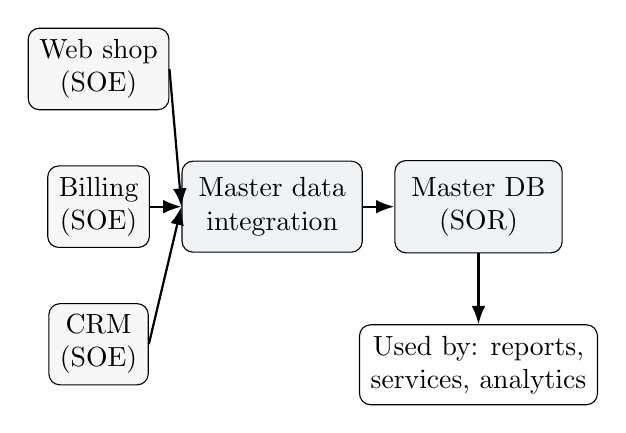
\begin{tikzpicture}[node distance=7mm]
\node[soft] (ws) {Web shop\\(SOE)};
\node[soft, below=of ws] (bill) {Billing\\(SOE)};
\node[soft, below=of bill] (crm) {CRM\\(SOE)};

\node[big, right=4mm of bill] (mdm) {Master data\\integration};

\node[big, right=4mm of mdm] (sor) {Master DB\\(SOR)};

\draw[arr] (ws.east) -- (mdm.west);
\draw[arr] (bill.east) -- (mdm.west);
\draw[arr] (crm.east) -- (mdm.west);
\draw[arr] (mdm.east) -- (sor.west);

\node[box, below=9mm of sor] (use) {Used by: reports,\\ services, analytics};
\draw[arr] (sor) -- (use);
\end{tikzpicture}

\vspace{0.4em}
\scriptsize In a \textbf{downstream} style, SOEs keep operating, and the SOR is built via integration rules.
\end{columns}
\end{frame}

\begin{frame}{From data warehouse to data lake}
\begin{itemize}
  \item Data warehouse: structured target schema, strong curation.
  \item Data lake: collect everything, structure later for use.
  \item Risk: \emph{data swamp} (unstructured pile without metadata discipline).
  \item Other hybrid ideas: \emph{data vault}, combining flexible data collection with more structure, traceability, and historical storage.
\end{itemize}
\end{frame}

\begin{frame}{Example: warehouse vs lake vs swamp}
\small
\begin{examplebox}[Scenario: online store analytics]
\small
We want to answer: \emph{``Which marketing campaigns lead to repeat purchases?''}
We have three kinds of data:
\begin{itemize}
  \item \textbf{Orders (OLTP tables)}: customer, order, payment, shipment
  \item \textbf{Clickstream logs}: page views, searches, add-to-cart events (often JSON)
  \item \textbf{Product reviews/images}: free text + media files
\end{itemize}
\end{examplebox}
\begin{block}{What changes between DW, lake, swamp?}
\begin{itemize}
  \item \textbf{Data warehouse:} we load \emph{clean, structured} tables
  (e.g., \texttt{FactSales}, \texttt{DimCustomer}, \texttt{DimTime}, \texttt{DimCampaign})
  so BI queries are fast and reliable.
  \item \textbf{Data lake:} we also store \emph{raw} logs and media first,
  and structure them when use case appears.
  \item \textbf{Data swamp (risk):} raw files are dumped without
  \textbf{metadata, ownership, versioning, or quality rules} $\Rightarrow$
  nobody trusts or can find the right data.
\end{itemize}
\end{block}

\end{frame}

% ============================================================
\section{Distribution}

\begin{frame}{Three-tier architecture (server architecture)}
\small
\begin{block}{Three tiers}
\begin{itemize}
  \item \textbf{Client tier} (front-end): UI for users
  \item \textbf{Logic tier} (application server): business logic, APIs
  \item \textbf{Data tier} (back-end): DBMS + database
\end{itemize}
\end{block}

\begin{examplebox}[Why thick-client and thin-client 2-tier styles often do not scale well]
\begin{itemize}
  \item \textbf{Thick client (logic on client):} hard to update and control (many installations), duplicated business rules, and clients often open many direct DB connections $\Rightarrow$ DB becomes the bottleneck.
  \item \textbf{Thin client (logic in DB / stored procedures):} business logic is tied to the database engine, harder to version/test, and scaling the DB tier is expensive; also encourages chatty client--DB traffic.
  \item \textbf{Three-tier helps:} one scalable middle tier can pool connections, cache, enforce security, and scale horizontally.
\end{itemize}
\end{examplebox}
\end{frame}

\begin{frame}{Three-tier architecture}
\small
\centering
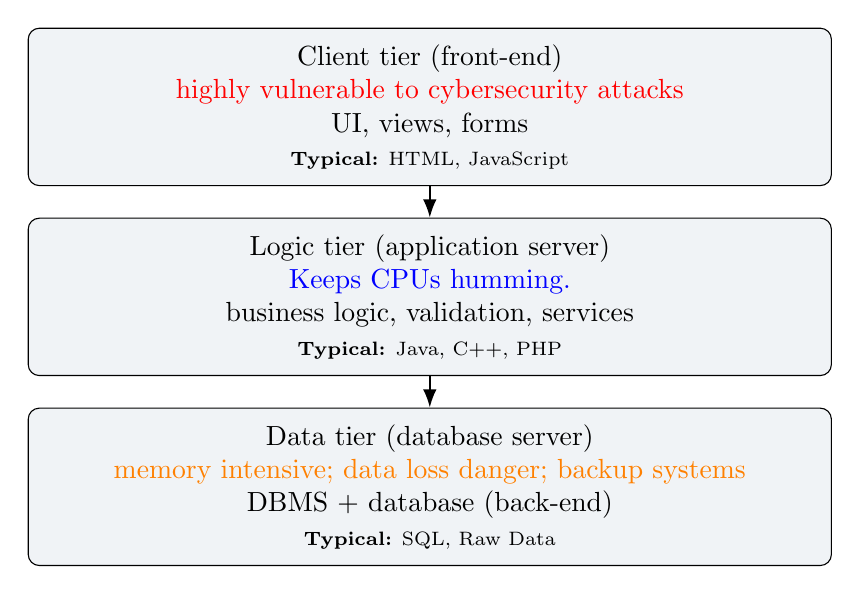
\begin{tikzpicture}[node distance=10mm]
\node[big, minimum width=10.2cm] (client) {Client tier (front-end)\\ \textcolor{red}{highly vulnerable to cybersecurity attacks}\\UI, views, forms\\
\scriptsize \textbf{Typical:} HTML, JavaScript};
\node[big, below=4mm of client, minimum width=10.2cm] (logic) {Logic tier (application server)\\
\textcolor{blue}{Keeps CPUs humming.}
\\business logic, validation, services\\
\scriptsize \textbf{Typical:} Java, C++, PHP};
\node[big, below=4mm of logic, minimum width=10.2cm] (data) {Data tier (database server)\\
\textcolor{orange}{memory intensive; data loss danger; backup systems}
\\DBMS + database (back-end)\\
\scriptsize \textbf{Typical:} SQL, Raw Data};
\draw[arr] (client) -- (logic);
\draw[arr] (logic) -- (data);
\end{tikzpicture}
\end{frame}



\begin{frame}{Parallel hardware architectures: overview}
\begin{itemize}
  \item \textbf{Shared disk}: multiple DB instances share the same storage.
  \item \textbf{Shared nothing}: DB is logically one, physically partitioned across nodes.
  \item \textbf{Shared memory}: many cores share the same RAM (common inside a node).
\end{itemize}
\end{frame}

\begin{frame}{Shared disk vs shared nothing}
\begin{columns}[T,onlytextwidth]
\column{0.5\textwidth}
\centering
\textbf{Shared disk}\\[0.3em]
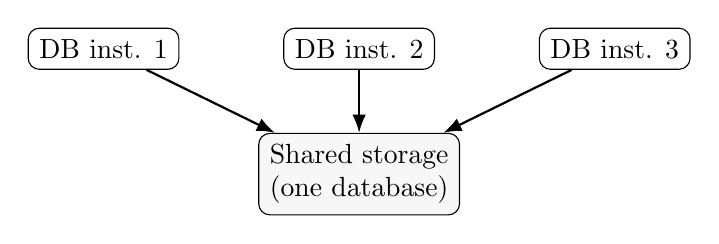
\begin{tikzpicture}[node distance=6mm, scale=0.95]
\node[soft] (db) {Shared storage\\(one database)};
\node[box, above left=8mm and 10mm of db] (n1) {DB inst. 1};
\node[box, above=8mm of db] (n2) {DB inst. 2};
\node[box, above right=8mm and 10mm of db] (n3) {DB inst. 3};
\draw[arr] (n1) -- (db);
\draw[arr] (n2) -- (db);
\draw[arr] (n3) -- (db);
\end{tikzpicture}

\column{0.5\textwidth}
\centering
\textbf{Shared nothing}\\[0.3em]
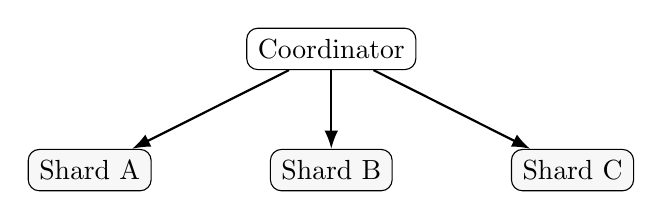
\begin{tikzpicture}[node distance=6mm, scale=0.95]
\node[box] (coord) {Coordinator};
\node[soft, below left=10mm and 12mm of coord] (s1) {Shard A};
\node[soft, below=10mm of coord] (s2) {Shard B};
\node[soft, below right=10mm and 12mm of coord] (s3) {Shard C};
\draw[arr] (coord) -- (s1);
\draw[arr] (coord) -- (s2);
\draw[arr] (coord) -- (s3);
\end{tikzpicture}
\end{columns}
\end{frame}


\begin{frame}{Replication vs sharding}
\begin{block}{Two ways to distribute data}
\begin{itemize}
  \item \textbf{Replication}: copy 100\% of data to multiple nodes.
  \item \textbf{Sharding}: split data among nodes (each stores a part).
\end{itemize}
\end{block}

\begin{itemize}
  \item Goals: \textbf{scalability} (horizontal/vertical) and \textbf{fault tolerance}.
  \item \textbf{Hash-based protocols} (e.g., consistent hashing) are commonly used to
  map keys to shards efficiently and keep rebalancing manageable when nodes join/leave.
  \item \textbf{Redundancy} (replication factor, erasure coding) helps prevent
  \textbf{inaccessibility} and \textbf{data loss} when disks or nodes fail.
  \item Typical large-scale systems that rely on sharding/partitioning ideas include
  \textbf{MapReduce/Hadoop} ecosystems (data split into blocks/partitions processed in parallel).
\end{itemize}
\end{frame}

\begin{frame}{Replication configurations}
\begin{columns}[T,onlytextwidth]
\column{0.5\textwidth}
\centering
\textbf{Master--slave (primary--secondary)}\\[0.3em]
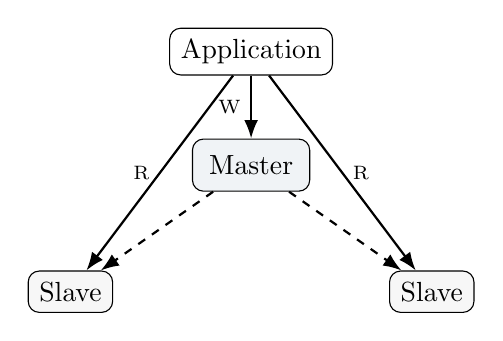
\begin{tikzpicture}[node distance=7mm]
\node[box] (app) {Application};
\node[big, below=8mm of app] (m) {Master};
\node[soft, below left=10mm and 10mm of m] (s1) {Slave};
\node[soft, below right=10mm and 10mm of m] (s2) {Slave};
\draw[arr] (app) -- node[left, font=\scriptsize]{W} (m);
\draw[arr] (app) -- node[left, font=\scriptsize]{R} (s1);
\draw[arr] (app) -- node[right, font=\scriptsize]{R} (s2);
\draw[arr, dashed] (m) -- (s1);
\draw[arr, dashed] (m) -- (s2);
\end{tikzpicture}

\column{0.5\textwidth}
\centering
\textbf{Peer-to-peer}\\[0.3em]
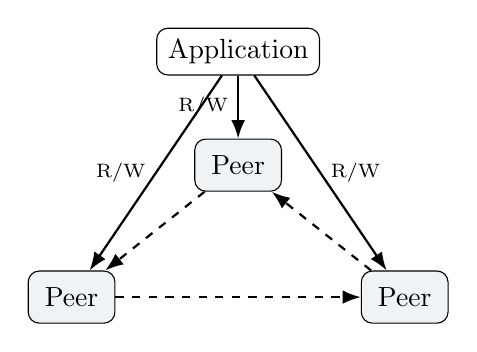
\begin{tikzpicture}[node distance=7mm]
\node[box] (app2) {Application};
\node[big, below=8mm of app2] (p1) {Peer};
\node[big, below left=10mm and 10mm of p1] (p2) {Peer};
\node[big, below right=10mm and 10mm of p1] (p3) {Peer};
\draw[arr] (app2) -- node[left, font=\scriptsize]{R/W} (p1);
\draw[arr] (app2) -- node[left, font=\scriptsize]{R/W} (p2);
\draw[arr] (app2) -- node[right, font=\scriptsize]{R/W} (p3);
\draw[arr, dashed] (p2) -- (p3);
\draw[arr, dashed] (p3) -- (p1);
\draw[arr, dashed] (p1) -- (p2);
\end{tikzpicture}
\end{columns}
\end{frame}

\begin{frame}{Synchronous vs asynchronous replication}
\begin{itemize}
  \item \textbf{Synchronous}: acknowledge write after other nodes (or quorum) replicate.
  \item \textbf{Asynchronous}: acknowledge write immediately; replicas catch up later.
\end{itemize}
\begin{examplebox}[Trade-off]
Synchronous improves consistency; asynchronous improves latency and availability.
\end{examplebox}
\end{frame}

\begin{frame}{Sharding + routing}
\centering
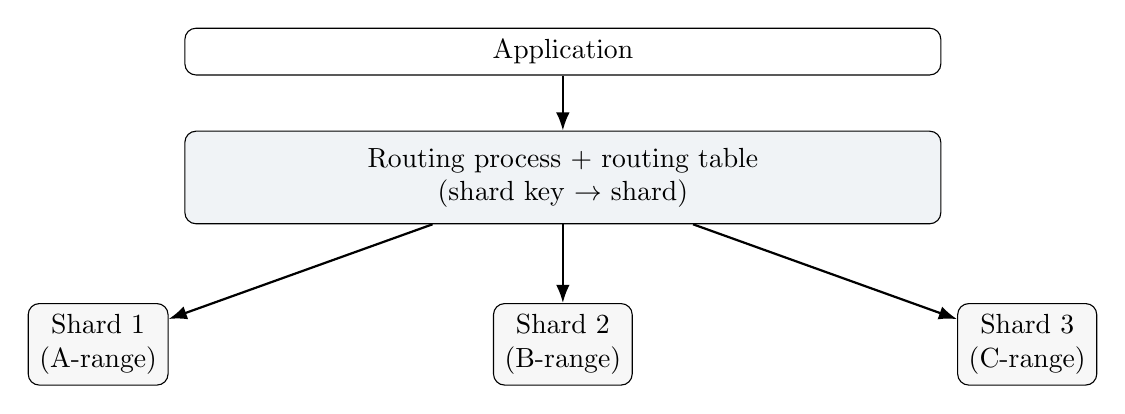
\begin{tikzpicture}[node distance=8mm]
\node[box, minimum width=9.6cm] (app) {Application};
\node[big, below=7mm of app, minimum width=9.6cm] (router) {Routing process + routing table\\(shard key \(\rightarrow\) shard)};
\node[soft, below left=10mm and 2mm of router] (sh1) {Shard 1\\(A-range)};
\node[soft, below=10mm of router] (sh2) {Shard 2\\(B-range)};
\node[soft, below right=10mm and 2mm of router] (sh3) {Shard 3\\(C-range)};
\draw[arr] (app) -- (router);
\draw[arr] (router) -- (sh1);
\draw[arr] (router) -- (sh2);
\draw[arr] (router) -- (sh3);
\end{tikzpicture}
\end{frame}

% ============================================================
\section{Database paradigms}

\begin{frame}{Database paradigms (data models)}
So far we focused on the relational paradigm. Other paradigms include:
\begin{itemize}
  \item Object-oriented databases (OODBMS)
  \item Object-relational DBMS (ORDBMS)
  \item NoSQL families: key-value, document, graph, column-family
\end{itemize}
\begin{examplebox}[Message]
Different models fit different needs; many systems are \emph{polyglot} (use several).
\end{examplebox}
\end{frame}

\begin{frame}{Object databases: key concepts}
\begin{itemize}
  \item Object: has unique identifier (OID), attributes, and state
  \item Encapsulation: methods + interface define behavior
  \item Class: set of objects with same attributes/methods
  \item Inheritance: subclasses/superclasses
\end{itemize}
\end{frame}

\begin{frame}{Object-relational impedance mismatch}
\scriptsize
\textit{Object-oriented applications organize data as objects with identity, methods, inheritance, and nested structure, whereas relational databases store data as tables, rows, and foreign keys. This difference is known as the \textbf{object-relational impedance mismatch}. Object-relational database systems aim to reduce this mismatch by extending the relational model with richer types and object-oriented features.}

\vspace{0.4em}

\begin{tabular}{@{}p{2.7cm}p{10.8cm}@{}}
\toprule
\textbf{Aspect} & \textbf{Mismatch between object-oriented and relational models} \\
\midrule
Encapsulation & Objects combine data and methods, while relational tables expose data only \\
Queries & Applications use navigational host-language logic, while databases use declarative SQL \\
Scopes & Objects enforce local visibility rules, whereas databases rely on global privileges and roles \\
Inheritance & Class hierarchies do not map naturally to flat relational tables \\
Structure & Objects may be nested or composite, while rows are typically flat tuples \\
Relationships & Object references and associations are more direct than foreign-key joins \\
Data types & Programming languages and DBMSs often support different type systems \\
\bottomrule
\end{tabular}
\begin{examplebox}[Interpretation]
ORDBMS tries to reduce mismatch while keeping relational foundations.
\end{examplebox}
\end{frame}




\begin{frame}{Big data challenges: the 6 V's (for self study)}
\small
NoSQL intuition often addresses scalability issues related to the 6Vs:
\begin{itemize}
  \item \textbf{Volume}: massive amounts of data
  \item \textbf{Velocity}: rapid data generation and updates
  \item \textbf{Variety}: heterogeneous data formats
  \item \textbf{Veracity}: uncertain or noisy data quality
  \item \textbf{Variability}: changing workloads and meanings
  \item \textbf{Value}: extracting useful benefit from data
\end{itemize}
\end{frame}

\begin{frame}{NoSQL intuition: relaxing strict consistency (for self study)}
\small
To cope with big data challenges, many distributed data systems
\textbf{relax the strictness and timing of consistency checks} in order
to improve scalability, fault tolerance, and availability.

\begin{block}{BASE}
\textbf{Basically Available, Soft state, Eventually consistent}

\medskip
\textbf{Soft state} means the system state may be temporarily inconsistent
and may change as replicas converge.
\end{block}

\begin{block}{CAP (intuition)}
Distributed systems often face trade-offs among
\textbf{Consistency}, \textbf{Availability}, and \textbf{Partition tolerance*}.
\end{block}

{\scriptsize *Partition tolerance means a distributed system keeps operating even when the network is split and some machines cannot communicate with others.}
\end{frame}

\begin{frame}{NoSQL families: four common paradigms}
\begin{itemize}
  \item \textbf{Key--value}: maps a key to a value; very fast lookups, but limited query capabilities
  \item \textbf{Document}: maps a key to a structured document (e.g.\ JSON or XML); supports queries within documents
  \item \textbf{Graph}: stores nodes, edges, and properties; efficient for relationship traversal
  \item \textbf{Column-family}: organizes data into keyspaces, column families, and rows with sparse columns
\end{itemize}
\end{frame}

\begin{frame}{Key-value model (not covered in lecture)}
\centering
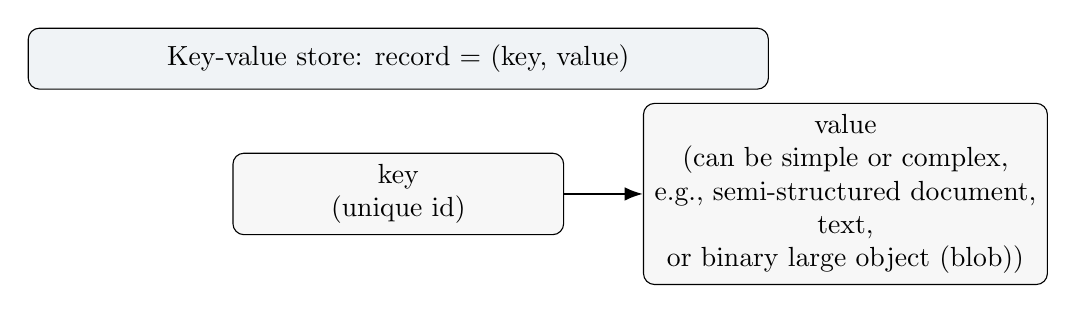
\begin{tikzpicture}[node distance=8mm]
\node[big, minimum width=9.4cm] (kv) {Key-value store: record = (key, value)};
\node[soft, below=8mm of kv, minimum width=4.2cm] (k) {key\\(unique id)};
\node[soft, right=10mm of k, minimum width=4.2cm] (v) {value\\(can be simple or complex,\\ e.g., semi-structured document,\\ text, \\or binary large object (blob))};
\draw[arr] (k) -- (v);
\end{tikzpicture}

\begin{block}{Query focus on keys}
Queries are guaranteed to be efficient for selections on keys. Limited query possibilities for values.    
\end{block}

\begin{block}{Lightweight and fast insert}
Easy to build and often used for real time or fast changing data, or document stores.
\end{block}

\end{frame}

\begin{frame}{Document model (JSON example (not covered in lecture))}
\scriptsize
\begin{examplebox}[A document (conceptual)]
\begin{tabular}{l}
\{\ \text{"customerID"}: "a800",\\
\quad \texttt{"name"}:\{\texttt{"first"}:"Matti",\ \texttt{"last"}:	exttt{\text{"Meikäläinen"}}\},\\
\quad \texttt{"address"}:\{\texttt{"street"}:"Kuja 2",\ \texttt{"zip"}:40100,\ \texttt{"city"}:"Jyväskylä"\},\\
\quad \texttt{"orders"}:[\{\texttt{"product"}:"Paahdin",\ \texttt{"qty"}:1\},\ \{\texttt{"product"}:"PC",\ \texttt{"qty"}:1\}]\\
\}
\end{tabular}
\end{examplebox}
\begin{itemize}
  \item DBMS understands document structure; can query nested fields.
\end{itemize}
\end{frame}

\begin{frame}{Graph model (not covered in lecture, for self study)}
\centering
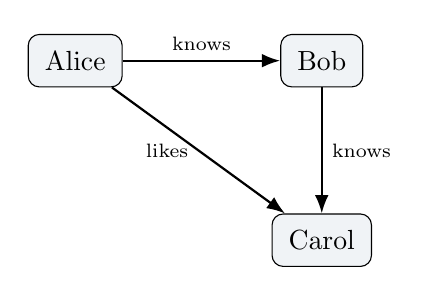
\begin{tikzpicture}[node distance=12mm]
\node[big] (a) {Alice};
\node[big, right=20mm of a] (b) {Bob};
\node[big, below=16mm of b] (c) {Carol};
\draw[arr] (a) -- node[above, font=\scriptsize]{knows} (b);
\draw[arr] (b) -- node[right, font=\scriptsize]{knows} (c);
\draw[arr] (a) -- node[left, font=\scriptsize]{likes} (c);

\end{tikzpicture}
\begin{itemize} 
 \item Edges are first-class: fast traversals for relationship-heavy queries. \item Supports graph queries such as path computation.
 \item Direct neighbors are fast accessible and easy/natural to query.
\end{itemize}
\end{frame}

\begin{frame}{Column-family model (not covered in lecture, for self study)}
\centering
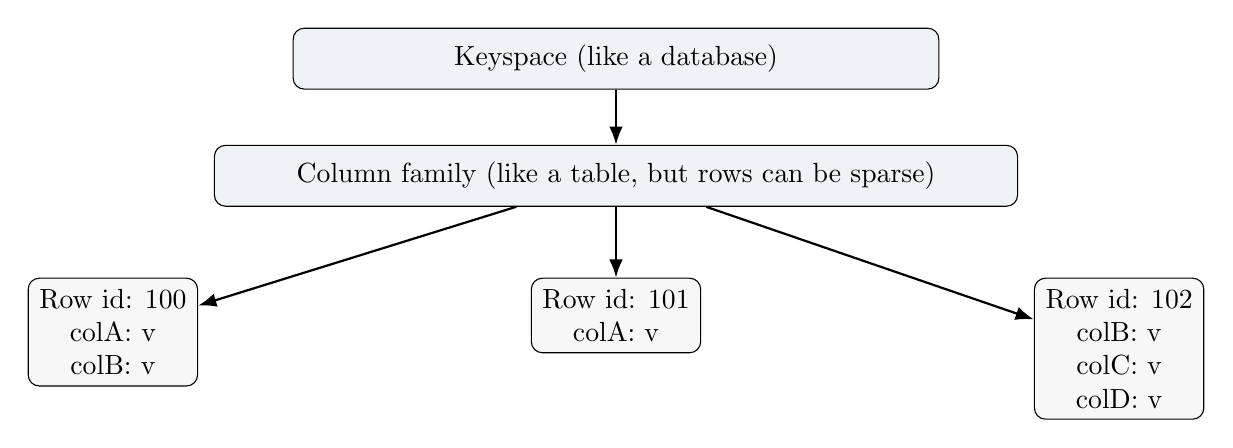
\begin{tikzpicture}[node distance=7mm]
\node[big, minimum width=8.2cm] (ks) {Keyspace (like a database)};
\node[big, below=7mm of ks, minimum width=10.2cm] (cf) {Column family (like a table, but rows can be sparse)};
\node[soft, below left=9mm and 2mm of cf] (r1) {Row id: 100\\colA: v\\colB: v};
\node[soft, below=9mm of cf] (r2) {Row id: 101\\colA: v};
\node[soft, below right=9mm and 2mm of cf] (r3) {Row id: 102\\colB: v\\colC: v\\colD: v};
\draw[arr] (ks) -- (cf);
\draw[arr] (cf) -- (r1);
\draw[arr] (cf) -- (r2);
\draw[arr] (cf) -- (r3);
\end{tikzpicture}
\end{frame}

\begin{frame}{Polyglot persistence (why “one DB” is not enough) (not covered in lecture, for self study)}
\begin{examplebox}[Online auction example idea]
Use different models for different subsystems:
\begin{itemize}
  \item payments: relational (strong correctness)
  \item recommendations: graph (fast joins/traversals)
  \item bids: key-value (speed)
  \item analytics: column-family / lake style (scale)
\end{itemize}
\end{examplebox}
\end{frame}

\begin{frame}{Relational vs NoSQL (typical trade-offs) (not covered in lecture, for self study)}
\scriptsize
\begin{tabular}{@{}p{3.6cm}p{5.6cm}p{5.2cm}@{}}
\toprule
 & \textbf{Relational} & \textbf{NoSQL (typical)} \\
\midrule
Query languages & Versatile & Simpler / domain-specific \\
Transactions & Strong (ACID) & Often weaker / BASE-style \\
Distribution & More laborious & Often easier / built-in \\
Use cases & General purpose & Specific domains \\
Reporting & Versatile & Often restricted \\
Maturity & Mature & Variable / newer \\
Cost & Free and commercial & Often free / mixed \\
Redundancy & Minimized & Tolerated / sometimes favored \\
\bottomrule
\end{tabular}
\end{frame}

% ============================================================
\section{Wrap-up}

\begin{frame}{Recap}
\begin{itemize}
  \item Data warehousing: ETL into a warehouse for reporting/OLAP/mining.
  \item DW schemas often use fact + dimension (star/snowflake/starflake).
  \item Distribution: three-tier architecture; parallel hardware patterns.
  \item Replication improves availability/fault tolerance; sharding improves scale.
  \item Beyond relational: object(-relational) and NoSQL families.
  \item Polyglot persistence: use the right model for each subsystem.
\end{itemize}
\end{frame}

\begin{frame}{Pointers}
\begin{itemize}
  \item This lecture is a summary of TIM Section 6 materials.
  \item For details, examples, and terminology, see the course page Section 6.
\end{itemize}
\end{frame}

\begin{frame}{Q\&A}
\begin{itemize}
  \item Where would you use a warehouse vs a lake?
  \item What would you replicate, what would you shard?
  \item Which paradigm fits your thesis/project domain?
\end{itemize}
\end{frame}

% --- Insert this slide near the end (e.g., right before Q&A)

\begin{frame}{Joke slide: The Babylonian Language Confusion (NoNoSQL)}
\small
Students, frustrated: \\
``Before NoSQL, we only had to learn SQL in the databases course.\\
Now, since NoSQL started, there are all kinds of languages and we have to learn them all!''

\vspace{0.6em}
\begin{columns}[T,onlytextwidth]
\column{0.58\textwidth}
\textbf{Student 1:} ``Let's start a counter movement!''\\[0.2em]
\textbf{Student 2:} ``How shall we name it?''\\[0.2em]
All Students: \textbf{``NoNoSQL``}

\vspace{0.6em}


\column{0.42\textwidth}
\centering
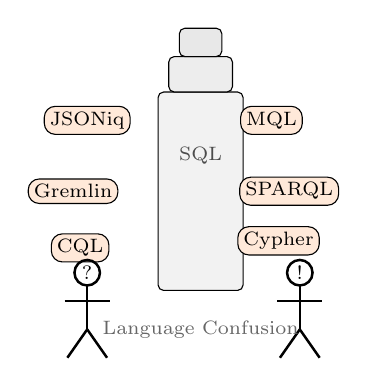
\begin{tikzpicture}[x=1cm,y=1cm,scale=0.9]
% tower
\draw[rounded corners=2pt, fill=black!5] (1.4,0.2) rectangle (2.6,3.0);
\draw[rounded corners=2pt, fill=black!7] (1.55,3.0) rectangle (2.45,3.5);
\draw[rounded corners=2pt, fill=black!9] (1.7,3.5) rectangle (2.3,3.9);
\node[font=\scriptsize, text=black!70] at (2.0,2.1) {SQL};

% scattered "languages" blocks
\foreach \x/\y/\t in {0.3/0.8/{CQL}, 0.2/1.6/{Gremlin}, 0.4/2.6/{JSONiq},
                     3.1/0.9/{Cypher}, 3.25/1.6/{SPARQL}, 3.0/2.6/{MQL}} {
  \node[draw,rounded corners,fill=JYUorange!15,inner sep=2pt,font=\scriptsize] at (\x,\y) {\t};
}

% stick students

\stick{0.4}{0.2}{?}
\stick{3.4}{0.2}{!}
\node[font=\scriptsize, text=black!60] at (2.0,-0.35) {Language Confusion};

\end{tikzpicture}
\end{columns}
\end{frame}
\end{document}